% !Mode:: "TeX:UTF-8"

\titlecontents{chapter}[2em]{\vspace{.5\baselineskip}\xiaosan\song}
             {\prechaptername\CJKnumber{\thecontentslabel}\postchaptername\qquad}{}
             {}             % 设置该选项为空是为了不让目录中显示页码
\addcontentsline{toc}{chapter}{中文译文}
\setcounter{page}{1}            % 单独从 1 开始编页码
\markboth{中文译文}{中文译文}   % 用于将章节号添加到页眉中
\chapter*{中文译文}
\textbf{摘要}

语义匹配是许多自然语言处理应用的一个基本问题, 它的目标在确定两个文本之间的匹配程度。近年来, 对这一问题采用了深入的学习方法, 并取得了显著的改进。在本文中, 我们建议将两个文本之间的全局交互的生成看作一个递归过程: 即两个文本在每个位置的相互作用是它们的前缀之间相互作用的组合, 以及词级交互当前位置。基于这个思想, 我们提出了一种新的深结构, 即Match-SRNN, 模型的递归匹配结构。首先, 构造张量来捕获单词级的相互作用。然后利用空间 RNN 递归的方式将局部相互作用结合起来, 以四种类型的门为重要。最后, 在全局交互的基础上计算匹配分数。我们表明, 在退化到精确匹配的情况下, Match-SRNN 可以逼近最长常见子序列的动态规划过程。因此, 对 SRNN 有一个明确的解释。我们对两个语义匹配任务的实验表明了Match-SRNN 的有效性, 以及它对所学匹配结构的可视化能力。

\textbf{介绍}

语义匹配是自然语言处理中许多应用的关键任务, 包括信息检索、问答和释义识别。语义匹配的目标是确定两个给定文本的匹配评分。

以问题回答的任务为例, 给出一对问题和答案, 建立匹配函数, 确定这两种文本之间的匹配度。传统的方法, 如 BM25 和基于特征的学习模式通常依赖于精确匹配模式来确定程度, 从而遭受词汇不匹配问题。

近年来, 深入学习的方法已经应用到这一领域, 并解决了词汇失配问题。现有的一些工作侧重于将每个文本表示为一个或多个稠密向量, 然后根据这些向量之间的相似性计算匹配分数。比如包括RAE、DSSM、CDSSM、ARC-I、CNTN、LSTM-RNN、MultiGranCNN 和 MV-LSTM。然而, 这些方法通常很难对两个 textsbecause 的复杂交互关系进行建模, 独立地计算表示形式。为了解决这一问题, 提出了一些深层次的方法来直接学习两种文本之间的交互关系, 包括 DeepMatch、ARC-II 和 MatchPyramid等。所有这些模型都通过分层匹配结构进行匹配: 两个文本之间的全局交互是不同级别的局部交互的组合, 如单词级别和短语级交互。

在所有这些方法中,两种文本之间复杂互动关系产生的机制尚不明确,因此缺乏可解释性。在本文中,我们建议以递归方式解决问题。具体而言,我们将全局交互的生成视为递归过程。给定两个文本$S_1\!\!=\!\!\{w_1,w_2,\cdots,w_m\}$ 和$S_2\!\!=\!\!\{v_1,v_2,\cdots,v_n\}$,每个位置的交互作用 $(i,j)$ (即$S_1[1{:}i]$和$ S_2 [1 {:} j] $之间的交互作用)前缀(即三次交互,$S_1[1{:}i{-}1]\!{\sim}\! S_2[1{:}j]$, $S_1[1{:}i]\!{\sim}\! S_2[1{:}j{-}1]$, $S_1[1{:}i{-}1]{\sim} S_2[1{:}j{-}1]$) ,以及在这个位置的字级交互(即$ w_i $和$ v_j $之间的交互),其中$S[1{:}c]$表示由前$ c $字文本组成的前缀$S$。与以前的层次匹配结构相比,递归匹配结构不仅可以捕获邻近词汇之间的相互作用,还可以考虑远距离的相互作用。

基于上述思想,我们提出了一种新颖的深层架构,即Match-SRNN来对递归匹配结构进行建模。首先,构造一个相似度张量来捕捉两个文本之间的单词级别的相互作用,其中每个元素表示来自不同文本的两个单词之间的相似性向量。然后将具有门控循环单元的空间(2D)递归神经网络(空间RNN)应用于张量。具体而言,每个位置$ \vec {h} _ {ij} $的表示可以被看作两个前缀之间的交互作用,即$ {S_1 [1 {:} i]} $和$ {S_2 [1 { :} j]} $。它由四个因素决定:$ \vec {h} _ {i-1,j},\vec {h} _ {i,j-1},\vec {h} _ {i-1,j-1 } $和输入字级交互$ \vec {s} _ {ij} $,分别取决于相应的门$ z_t,z_l,z_d $和$ z_i $。最后,由上述空间RNN获得的全局交互$ \vec {h} _ {mn} $表示的线性评分函数产生匹配分数。

我们证明Match-SRNN可以很好地逼近最长公共子序列(LCS)问题的动态规划过程。 此外,我们的仿真实验表明,通过回溯每个位置处的最大的门可以获得清晰的匹配路径,类似于LCS中的最长公共子序列。 因此,关于Match-SRNN中如何生成全局交互的清晰解释。

我们对问题回答和论文引用任务进行了实验,以评估我们模型的有效性。

实验结果表明, SRNN 能显著优于现有的深度模型。同时, 为了对所学匹配结构进行可视化, 给出了从实际数据中抽取的两个文本的匹配路径。

本文的贡献可以概括为:
\begin{itemize}
\item 递归地构建语义匹配机制的思想,即递归匹配结构。
\item 提出了一种新的深层架构,即Match-SRNN,来对递归匹配结构进行建模。 实验结果表明,与现有的深度模型相比,Match-SRNN可以显着提高语义匹配的性能。
\item Match-SRNN与LCS之间关系的揭示,即〜Match-SRNN可以在完全匹配的场景中再现LCS的匹配路径。
\end{itemize}

\textbf{相关工作}

现有的用于语义匹配的深度学习方法可以分成两组。

一个范例着重于将每个文本表示为密集向量,然后根据这两个向量之间的相似度计算匹配分数。例如,DSSM〜\ cite {huang2013learning}使用多层全连接神经网络将查询(或文档)编码为矢量。
CDSSM和ARC-I采用卷积神经网络(CNN),而LSTM-RNN采用长时间短的递归神经网络长期记忆(LSTM)单位更好地代表一个句子。
与上述工作不同的是,CNTN使用神经张量网络来模拟两个句子之间的相互作用,而不是使用余弦函数。通过这种方式,它可以捕获更复杂的匹配关系。有些方法甚至尝试将两个句子与多个表示进行匹配,例如单词,短语和句子级别表示。例子包括RAE,BiCNN,MultiGranCNN和MV-LSTM。一般而言,这种方法背后的想法与用户的经验是一致的,即一旦两句话的含义被很好地捕捉,就可以确定两句之间的匹配程度。然而,这些方法通常很难模拟两个文本之间复杂的相互作用关系,特别是当它们已经被表示为一个紧凑的向量。

另一个范式转向直接模拟两个文本的交互关系。具体而言,交互被表示为密集向量,然后通过整合这种交互来产生匹配分数。这种范式的大多数现有工作都创建了一个层次匹配结构,即〜两个文本之间的全局交互是通过分层合成本地交互来生成的。
例如,DeepMatch将两个文本之间全局交互的生成模型化为基于主题层次结构的本地交互。 MatchPyramid使用CNN将全局交互的生成模型化为单词级别和短语级别交互的抽象。由于分层匹配结构通常依赖于组合的固定窗口大小,所以在这种模型中不能很好地捕获局部交互之间的长距离依赖关系,因此分层定义匹配结构具有局限性。

\textbf{循环匹配结构}

在所有现有的方法中,语义匹配的机制复杂且难以解释。
在数学和计算机科学中,当面对一个复杂的对象时,简化的一种常见方法是将问题分成同类型的子问题,并试图递归地解决问题。 这是众所周知的递归思想。 在本文中,我们建议递归地解决语义匹配问题。
%
%%%%%%%%
%


\textbf{Match-SRNN}

在本节中,我们介绍一种新的深层架构,即Match-SRNN,以对递归匹配结构进行建模。 如图~\ref{fig:architecture}所示,Match-SRNN由三部分组成:
(1)一个神经张量网络来捕捉单词级别的相互作用; (2)应用于单词相互作用张量的空间RNN以获得全局交互; (3)获得最终匹配分数的线性评分函数。

\textbf{神经张量网络}
在Match-SRNN中,首先利用神经张量网络来捕捉两个文本之间的基本交互,即词级交互。
具体而言,每个单词首先被表示为分布式向量。 给定任意两个单词$ w_i $和$ v_j $,以及它们的向量$ u(w_i)$和$ u(v_j)$,它们之间的交互可以表示为一个向量:
\begin{equation*}
\vec{s}_{ij}=F(u(w_i)^TT^{[1:c]}u(v_j)+W\begin{bmatrix}
		u(w_i)\\
		u(v_j)
	\end{bmatrix}+\vec{b}),
\end{equation*}
其中$ T ^ i,i \ in [1,...,c] $是张量参数的一个片段,$ W $和$ \ vec {b} $是线性部分的参数。 $ F $是一个非线性函数,本文使用整流器$ F(z)= \ max(0,z)$。

交互也可以表示为相似性分数,如余弦。 我们在这里采用神经张量网络,因为它可以捕捉更复杂的相互作用。
\begin{figure}[!htbp]
\vspace{1em}
\centering
  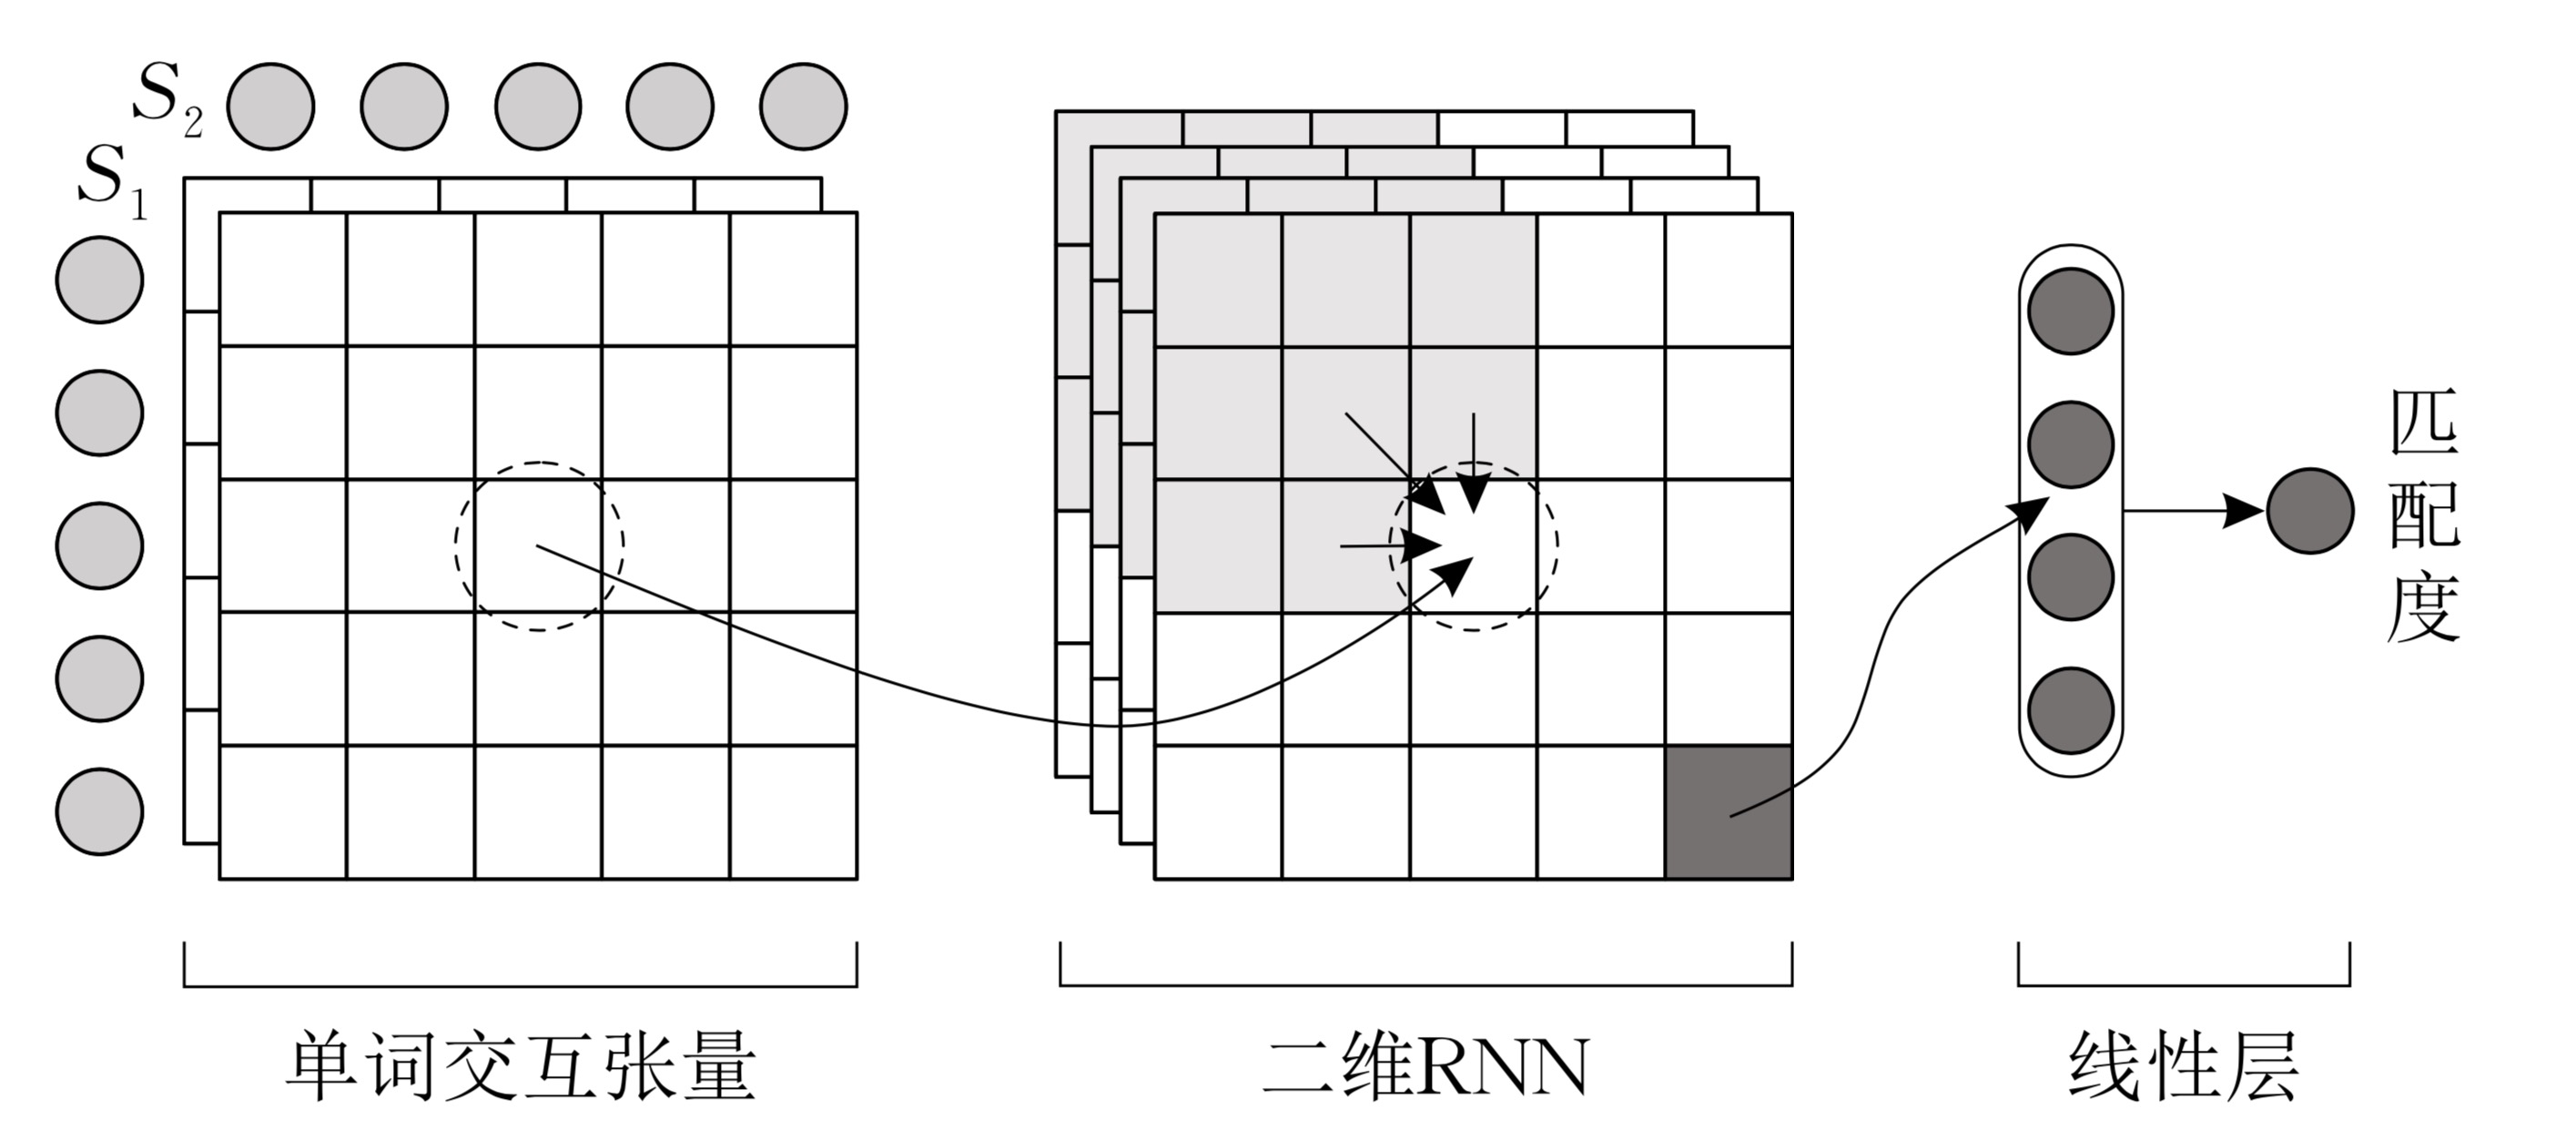
\includegraphics[width=0.9\linewidth]{figures/MatchSRNN.jpg}
  \caption{MatchSRNN模型}
  \label{fig:architecture}       % Give a unique label
\vspace{1em}
\end{figure}



\textbf{空间RNN}
Match-SRNN的第二步是将空间RNN应用于词级交互张量。 Spatial RNN,也被称为二维RNN(2D-RNN),是多维RNN的特例。 根据空间RNN,给定前缀的交互表示:$S_1[1{:}i{-}1]\!{\sim}\! S_2[1{:}j]$, $S_1[1{:}i]\!{\sim}\! S_2[1{:}j{-}1]$和$S_1[1{:}i{-}1]\!{\sim}\! S_2[1{:}j{-}1]$表示为$\vec{h}_{i-1,j},\vec{h}_{i,j-1}$, 
\begin{equation}
\vec{h}_{ij}=f(\vec{h}_{i-1,j},\vec{h}_{i,j-1},\vec{h}_{i-1,j-1},\vec{s}_{ij}).
\end{equation}

因此,我们可以看到,空间RNN可以自然地对方程式(\ ref {eq:RecursiveMatchStruct})中定义的递归匹配结构进行建模。

对于函数$ f $,我们有不同的选择。基本RNN通常使用非线性全连接层作为$ f $。这种类型的函数易于计算,但经常会遇到渐变消失和爆炸问题〜\ cite {DBLP:conf / icml / PascanuMB13}。因此,已经提出了RNN的许多变体,诸如长期短期记忆(LSTM),门控重复单元(GRU)和网格LSTM。在这里,我们采用GRU,因为它很容易实现,并且与LCS有着密切的关系,这将在下面的章节中讨论。

GRU被提议利用几个门来解决上述的基本RNN问题,并且已经在诸如机器翻译等任务中表现出优异的性能。在本文中,我们将序列(1D-GRU)的传统GRU扩展到空间GRU。

对于1D-GRU,给定一个句子$ S {=}(x_1,x_2,\cdots,x_T)$,其中$ \vec {x} _t $表示嵌入$ t $个词,位置$ t $,即$ \vec {h} _t $,可以计算如下:
\begin{equation*}
	\begin{aligned}
		\vec{z} \,& {=} \sigma(W^{(z)}\vec{x}_t + U^{(z)}\vec{h}_{t-1}),\,\vec{r}{=} \sigma(W^{(r)}\vec{x}_t + U^{(r)}\vec{h}_{t-1}), \\
		\vec{h}'_t \,&{=} \phi(W\vec{x}_t{+}U(\vec{r}\odot \vec{h}_{t-1})),\,\vec{h}_t{=} (\vec{1}-\vec{z})\odot \vec{h}_{t-1} {+} \vec{z} \odot \vec{h}'_t,
	\end{aligned}
\end{equation*}

其中$ \vec {h} _ {t-1} $表示 $t{-}1$的位置$W^{(z)},U^{(z)},W^{(r)},U^{(r)},W$和$ U $是参数,$ \vec {z} $是更新门,它试图控制是将旧信息传播到新状态还是写新 生成的信息到状态,$ \vec {r} $是重置门,当产生新的候选隐藏状态时,它试图重置存储在单元中的信息。

当扩展到空间GRU时,对于给定位置$(i,j)$,即〜$(i { - } 1,j),(i,j { - } 1)$和$ (i { - } 1,j { - } 1)$,因此我们将有四个更新门$ \vec {z} $,记为$ \vec {z} _ {l},\vec {z} _t ,\vec {z} _d $和$ \vec {z} _i $以及三个复位门$ \vec {r} $,记为$\vec{r}_l, \vec{r}_t, \vec{r}_d$。 函数$ f $计算如下。

\begin{align}\label{eq:SRNN}
&\vec{q}^T=[\vec{h}_{i-1,j}^T,\vec{h}_{i,j-1}^T,\vec{h}_{i-1,j-1}^T,\vec{s}_{ij}^T]^T,\nonumber\\
		&\vec{r}_l =\sigma(W^{(r_l)}\vec{q}+\vec{b}^{(r_l)}),\,\vec{r}_t =\sigma(W^{(r_t)}\vec{q}+\vec{b}^{(r_t)}),\nonumber\\
		&\vec{r}_d =\sigma(W^{(r_d)}\vec{q}+\vec{b}^{(r_d)}),\,\vec{r}^T  =[\vec{r}_l^T,\vec{r}_t^T,\vec{r}_d^T]^T,\nonumber\\
		&\vec{z}'_{i} = W^{(z_i)}\vec{q}+\vec{b}^{(z_i)},\,\vec{z}'_{l} =W^{(z_l)}\vec{q}+\vec{b}^{(z_l)},\nonumber\\
 		&\vec{z}'_{t} =W^{(z_t)}\vec{q}+\vec{b}^{(z_t)},\,\vec{z}'_{d}=W^{(z_d)}\vec{q}+\vec{b}^{(z_d)},\nonumber\\
 		&[\vec{z}_i, \vec{z}_l, \vec{z}_t, \vec{z}_{d}] = \texttt{SoftmaxByRow}([\vec{z}'_i, \vec{z}'_l, \vec{z}'_t, \vec{z}'_{d}]),\\
 		&\vec{h}'_{ij} {=}\phi(W\vec{s}_{ij} + U(\vec{r}\odot[\vec{h}_{i,j-1}^T, \vec{h}_{i-1,j}^T, \vec{h}_{i-1,j-1}^T]^T) + \vec{b}), \nonumber\\
 		&\vec{h}_{ij}     {=}\vec{z}_{l}\odot\vec{h}_{i,j-1}{+}\vec{z}_{t}\odot\vec{h}_{i-1,j}{+}
            		  \vec{z}_{d}\odot\vec{h}_{i-1,j-1}{+}\vec{z}_{i}\odot\vec{h}'_{ij},
	\end{align}

\textbf{线性打分函数}
由于空间RNN是从左上角到右下角扫描输入的递归模型,因此我们可以在右下角获得最后一个表示为$ \vec {h} _ {mn} $。 $ \vec {h} _ {mn} $反映了两个文本之间的全局交互。 最终的匹配分数可以用线性函数获得:
\begin{equation}
M(S_1,S_2)=W^{(s)}\vec{h}_{mn}+\vec{b}^{(s)},
\end{equation}
其中 $W^{(s)}$ 和 $\vec{b}^{(s)}$代表参数。

\textbf{优化}
对于不同的任务,我们需要利用不同的损失函数来训练我们的模型。
以回归为例,我们可以使用平方损失进行优化:
\begin{equation}
\mathcal{L}(S_1,S_2,y)= (y-M(S_1,S_2))^2,
\end{equation}
其中 $y\in R$是指示$S_1$ 和$S_2$ 之间匹配程度的实值地面真值标签

对于排序问题,我们可以利用转折点损失等成对排序损失进行训练。 给定一个三元$(S_1,S_2 ^ +,S_2 ^ - )$,其中$(S_1,S_2 ^ +)$的匹配度高于$(S_1,S_2 ^ - )$,损失函数定义为:
\begin{equation*}
\mathcal{L}(S_1, S_2^+, S_2^-) = \max(0, 1-M(S_1, S_2^+)+M(S_1, S_2^-))
\end{equation*}

其中,$M(S_1,S_2^+)$ 和 $M(S_1,S_2^-)$ 是匹配一致性打分。

通过反向传播和随机梯度下降联合训练模型的所有参数,包括词嵌入参数,神经张量网络,空间RNN。 具体来说,我们在训练过程中的所有参数上使用AdaGrad。

\textbf{讨论}

在本节中,我们将展示Match-SRNN与众所周知的最长公共子序列(LCS)问题之间的关系。

\textbf{理论分析}
最长公共子序列问题的目标是找到一组序列中所有序列共有的最长子序列(通常只有两个序列)。 在诸如DNA检测的许多应用中,最长公共子序列的长度被用于定义两个序列之间的匹配程度。 %这个问题在多项式时间内可以通过动态规划解决,因为它具有最优的子结构。

形式上来说,给定两个序列,如:$S_1{=}\{x_1,\cdots,x_m\}$和$S_2{=}\{y_1,\cdots,y_n\}$, 使 $c[i,j]$ 代表的是$S_1[1{:}i]$ and $S_2[1{:}j]$的最长公共子序列长度。$S_1$ 和$S_2$的最长公共子序列长度通过下述的循环过程获得。每一步$c[i,j]$ 由四个因素决定: $c[i{-}1,j{-}1],c[i{-}1,j],c[i,j{-}1]$ ,以及$x_i$ 和 $y_j$是否一样。
\begin{equation}\label{eq:LCS}
c[i,j]{=}\max(c[i,j{-}1], c[i{-}1,j],c[i{-}1,j{-}1]+\mathbb{I}_{\{x_i=y_j\}}),
\end{equation}
其中,$\mathbb{I}_{\{x_i=y_j\}}$是一个指示符函数,当$x_i=y_j$,函数为1,否则为0。$i{=}0$ 或 $j{=}0$时,$c[i,j]{=}0$。

Match-SRNN与LCS有很强的连接。 为了表明这一点,我们首先退化Match-SRNN来模拟精确匹配问题,用一个简单的指标函数代替神经张量网络,如果两个词完全相同则返回1,否则返回0,即$ s_ {ij} {=}\mathbb{I}_ {\{X_I= y_j\}}$。
空间GRU单元的尺寸也被设置为1.空间GRU的复位门被禁用,因为LCS的长度根据所有过去的历史累积。 因此,等式(4)可以退化为
\[
{h}_{ij}     ={z}_{l}\cdot{h}_{i,j-1}+{z}_{t}\cdot{h}_{i-1,j}+
            		  {z}_{d}\cdot{h}_{i-1,j-1}+{z}_{i}\cdot{h}'_{ij},
\]

\textbf{模拟结果}
我们进行了一个模拟实验来验证上面显示的分析结果。 该数据集由许多随机抽样序列对构成,每个序列由从词汇\textit {\{A B C D E F G H I J \}}中抽样的字符组成。 首先,对每个序列对进行LCS的动态规划算法,将LCS的归一化长度设置为每个序列对的匹配程度。 为了仿真,我们将数据分成训练(10000对)和测试集(1000对),并训练带有回归损失的Match-SRNN。 两个序列$ S_1 = \{A,B,C,D,E \} $和$ S_2 = \{F,A,C,G,D \} $的仿真结果如图~\ref{fig:simulation}所示。

图~\ref{fig:simulation}(a)显示了LCS的结果,其中每个位置的得分$(i,j)$代表$ c [i,j] $,灰色路径指示通过回溯动态编程过程获得两个序列之间的LCS。 (b)给出了Match-SRNN的结果,其中每个位置处的分数$(i,j)$代表表示$ \ vec {h} _ {ij} $(请请注意,为了简化,$ \ vec {h} _ {ij} $的维度被设置为$ 1 $)。我们可以看到Match-SRNN产生的分数与LCS获得的分数相同,这揭示了Match-SRNN和LCS之间的关系。

图~\ref{fig:simulation}(b)中的灰色路径显示了本地交互如何合成全局交互的主要途径,
是通过回溯门产生的。图3(c)显示了路径生成过程,其中每个位置的三个值代表三个门,例如$ z_l {=} 0.9,z_t {=} 0.1,z_d {=}$位置$(5,5)$处为$ $。考虑到最后位置$(5,5)$,匹配信号从具有最大门值的方向(即〜$ z_l $)传递过来,因此,我们移动到位置$(5,4)$。在位置$(5,4)$,门的最大值是$ z_d {=} 0.7 $,因此,我们应该移动到位置$(3,3)$。我们可以看到Match-SRNN引起的路径与动态编程的路径相同。该分析给出了Match-SRNN如何解决语义匹配问题的机制。
\begin{figure}[t]
\centering
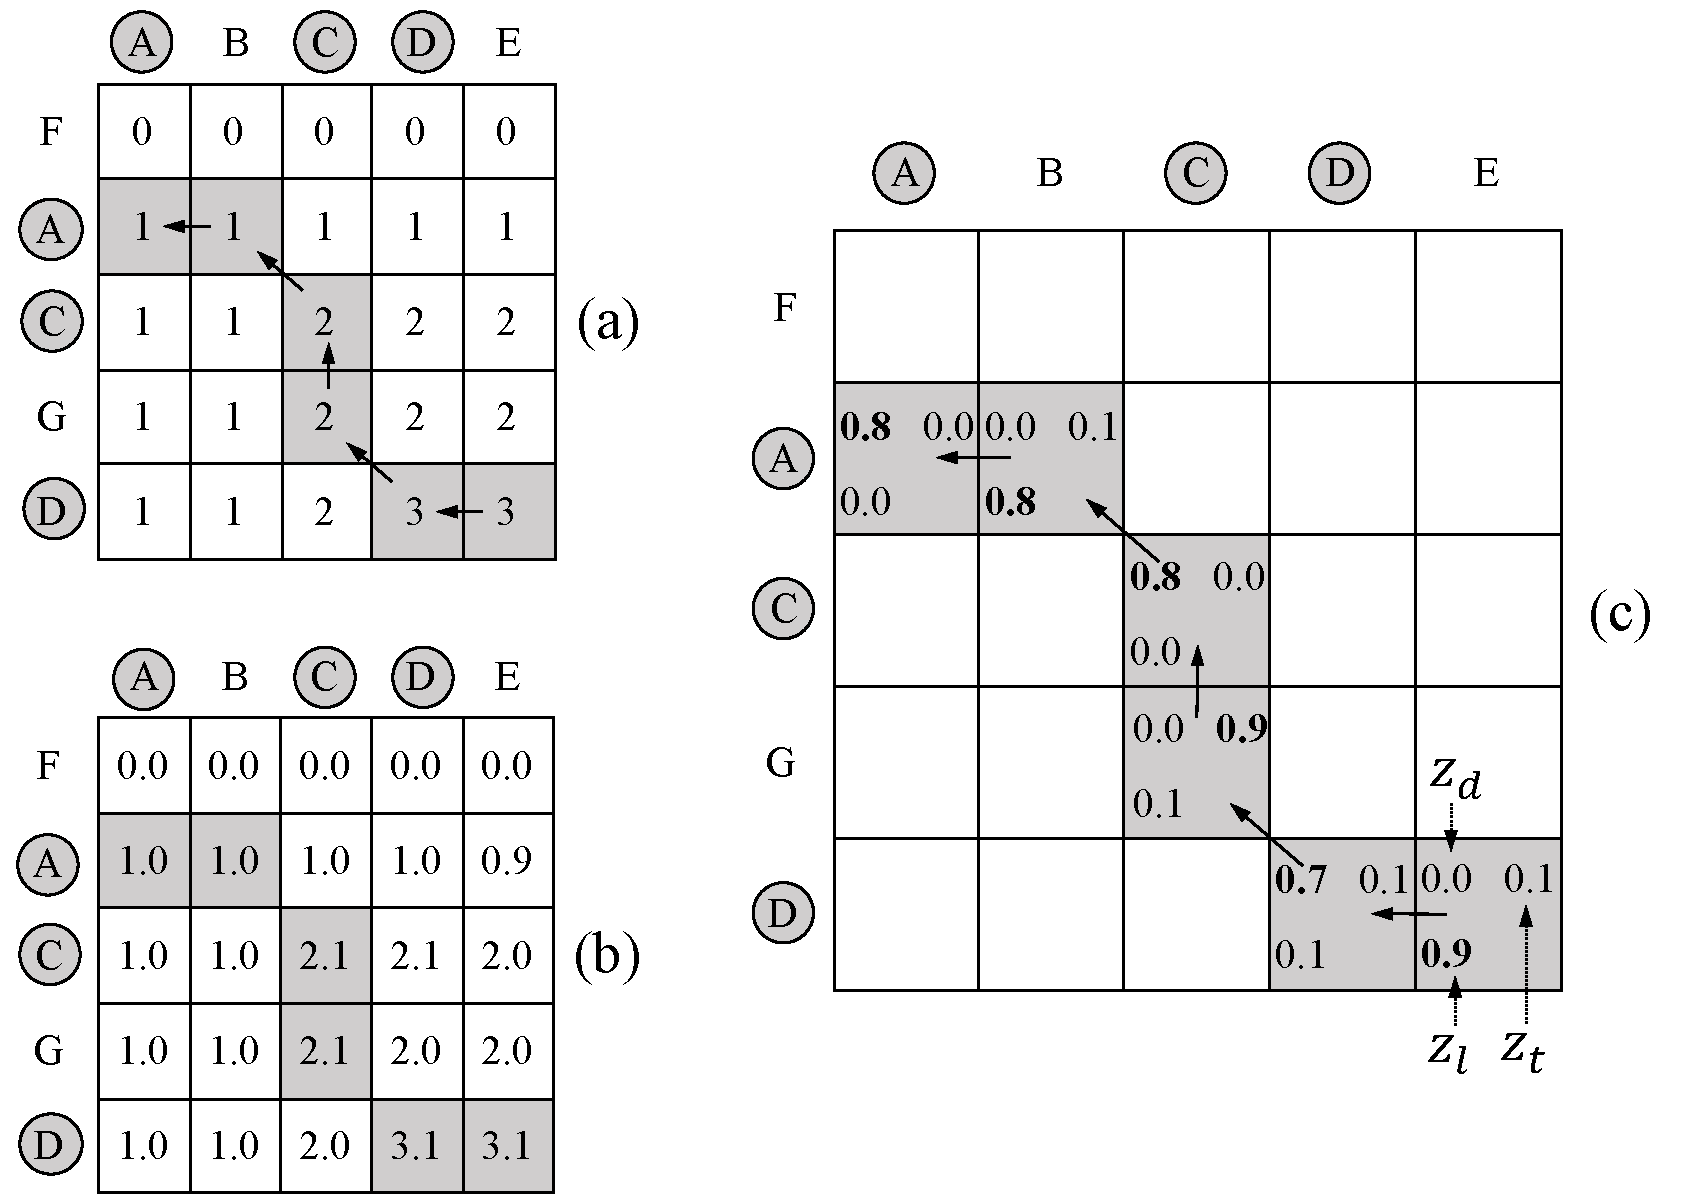
\includegraphics[width=0.7\textwidth]{figures/lcs_simulation_more.pdf}
\caption{Match-SRNN的LCS仿真结果。 图(a)显示了在LCS中发现的匹配度和路径。 图(b)显示了Match-SRNN的模拟结果。 图(c)显示了在Match-SRNN中找到灰色路径的回溯过程。}\label{fig:simulation}
%\label{fig:model}
\end{figure}


\textbf{实验}

我们对问答(QA)和论文引用(PC)的任务进行了实验,以评估Match-SRNN的有效性。

QA数据集收集自Yahoo!解答,社区问答系统,一些用户向系统提出问题,其他用户将提交他们的答案。
整个数据集包含142,627(问题,答案)对,每个问题都伴随着最佳答案。
我们选择其中问题和他们的最佳答案都长度在5到50之间的对。
之后,数据集包含60,564个(问题,答案)对,它们形成正对。对于每个问题,我们首先使用其最佳答案作为查询,用Lucene搜索引擎从整个答案集中检索前1000个结果。然后我们从它们中随机选择4个答案来构造负对。 %我们将整个数据集与8:1:1比例的训练数据,验证数据和测试数据分开。

PC任务是将两篇论文与引文关系进行匹配。
该数据集按照MatchPyramid构建。
论文摘要信息和引文网络是从商业学术网站​​收集的。
%我们使用每张纸的摘要作为匹配的文本。
负数对从整个数据集中随机抽样。
最后,我们有280K积极和560K消极情况。

\textbf{Match-SRNN的效果}
我们比较了Match-SRNN和几种现有的深度学习方法,包括ARC-I,ARC-II,CNTN,LSTM-RNN,MultiGranCNN,MV-LSTM和MatchPyramid。我们还将其与BM25〜\ cite {robertson1995okapi}进行了比较,这是一种在信息检索中用于语义匹配的流行且强大的基准。对于Match-SRNN,我们还实现了双向版本进行比较,它也从右下到左上扫描词相互作用张量,表示为双匹配-SRNN。

在我们的实验中,我们设置参数和基线如下。
在我们的模型和一些基线深度模型中使用的词嵌入全部由\texttt {Word2Vec} 的\texttt {SkipGram}初始化。
根据前面的练习,在整个问题答案数据集上训练词嵌入,并将维数设置为50。
SGD的批量大小设置为128.所有其他可训练参数均以相同比例的均匀分布进行随机初始化,并根据验证集上的性能进行选择。 AdaGrad的初始学习率也通过验证来选择。神经张量网络和空间RNN的维数设为10,因为它在$ d = 1,2,5,10,$和$ 20 $的设置中获得了最佳验证结果。基线方法的其他参数是通过从原始文件中获取值来设置的。

质量保证任务被制定为排名问题。因此,我们使用铰链损失进行优化,如第4.4节所示,并且通过典型的排名测量来评估结果,例如Precision为1(表示为P1)和Mean Reciprocal Rank(MRR)。
\begin{equation*}
P@1=\frac{1}{N}\sum_{i=1}^{N}\delta(r(S_2^{+(i)})= 1),\,
MRR=\frac{1}{N}\sum_{i=1}^{N}\frac{1}{r({S_{2}^{+(i)}})},
\end{equation*}
其中$ N $是测试排名列表的数量,$ S_2 ^ {+(i)} $是第i个排名列表中的正数句子,$ r(\cdot)$表示在 排名列表和$ \delta $是指标函数。
PC任务被制定为二进制分类任务。 因此匹配分数由softmax层使用,交叉熵损失用于训练。
我们使用分类准确性(Acc)作为评估指标。

\begin{table}[t]
%\begin{tabular*}{0.435\textwidth}{c|cc} \hline
\begin{tabular}{l|cc|c} \hline
&
\multicolumn{2}{c|}{QA} &
\multicolumn{1}{c}{PC} \\ \hline
\multicolumn{1}{c|}{Model} &
\multicolumn{1}{c}{P@1} &
\multicolumn{1}{c|}{MRR} &
\multicolumn{1}{c}{Acc} \\ \hline
Random Guess			& 0.200 & 0.457 & 0.500   \\
BM25        			& 0.579 & 0.726 & 0.832	    \\ \hline
ARC-I 					& 0.581 & 0.756 	& 0.845	\\
CNTN					& 0.626 & 0.781 	& 0.862 	\\
LSTM-RNN   		  		& 0.690 	& 0.822 	& 0.878 	\\ \hline
%RAE	 					& 0.398 & 0.652	& *	\\
MultiGranCNN			& 0.725 	& 0.840 & 0.885		\\
MV-LSTM  				& 0.766	& 0.869	& 0.890	\\ \hline
%DeepMatch  				& 0.452 & 0.679	& *	\\
ARC-II 					& 0.591 & 0.765 	& 0.865	\\
MatchPyramid-Tensor			& 0.764 & 0.867 	& 0.894\\ \hline
% Match-LSTM  			& 0.768 & 0.870		\\
% Match-LSTM (dynamic)  	& 0.782 & 0.878		\\
Match-SRNN 				& 0.785 & 0.879 & 0.898 \\
Bi-Match-SRNN  			& \textbf{0.790}	& \textbf{0.882} 	& \textbf{0.901}	\\
\hline
\end{tabular}
\centering
\caption{QA 和 PC 任务上的实验结果.}\label{tab:results}
\end{table}

实验结果列于Table\ref{tab:results}。我们有以下实验结果:

(1)通过对递归匹配结构进行建模,Match-SRNN与所有基线相比可显着提高性能。
以QA任务为例,与BM25相比,以P $@$ 1为例,改进约为36.4\%。
与MV-LSTM相比,以学习句子表示为主的深度学习方法中最好的一种,其改进约为3.1\%。

对于PC任务,Match-SRNN也取得了最佳效果,但与QA任务相比,这些改进较小。这是因为这项任务比较容易,甚至像BM25这样简单的模型都能产生好的结果。从以上分析可以看出,递归匹配结构有助于提高语义匹配的结果。

(2)两种匹配范式(将文本表示为密集向量并将相互作用关系建模)都有其自身的优势,并且结果具有可比性,例如~QA数据集上两种范式的先前最佳结果分别为0.766 / 0.869( MV-LSTM)和0.764 / 0.867(MatchPyramid)。

\begin{figure}[t]
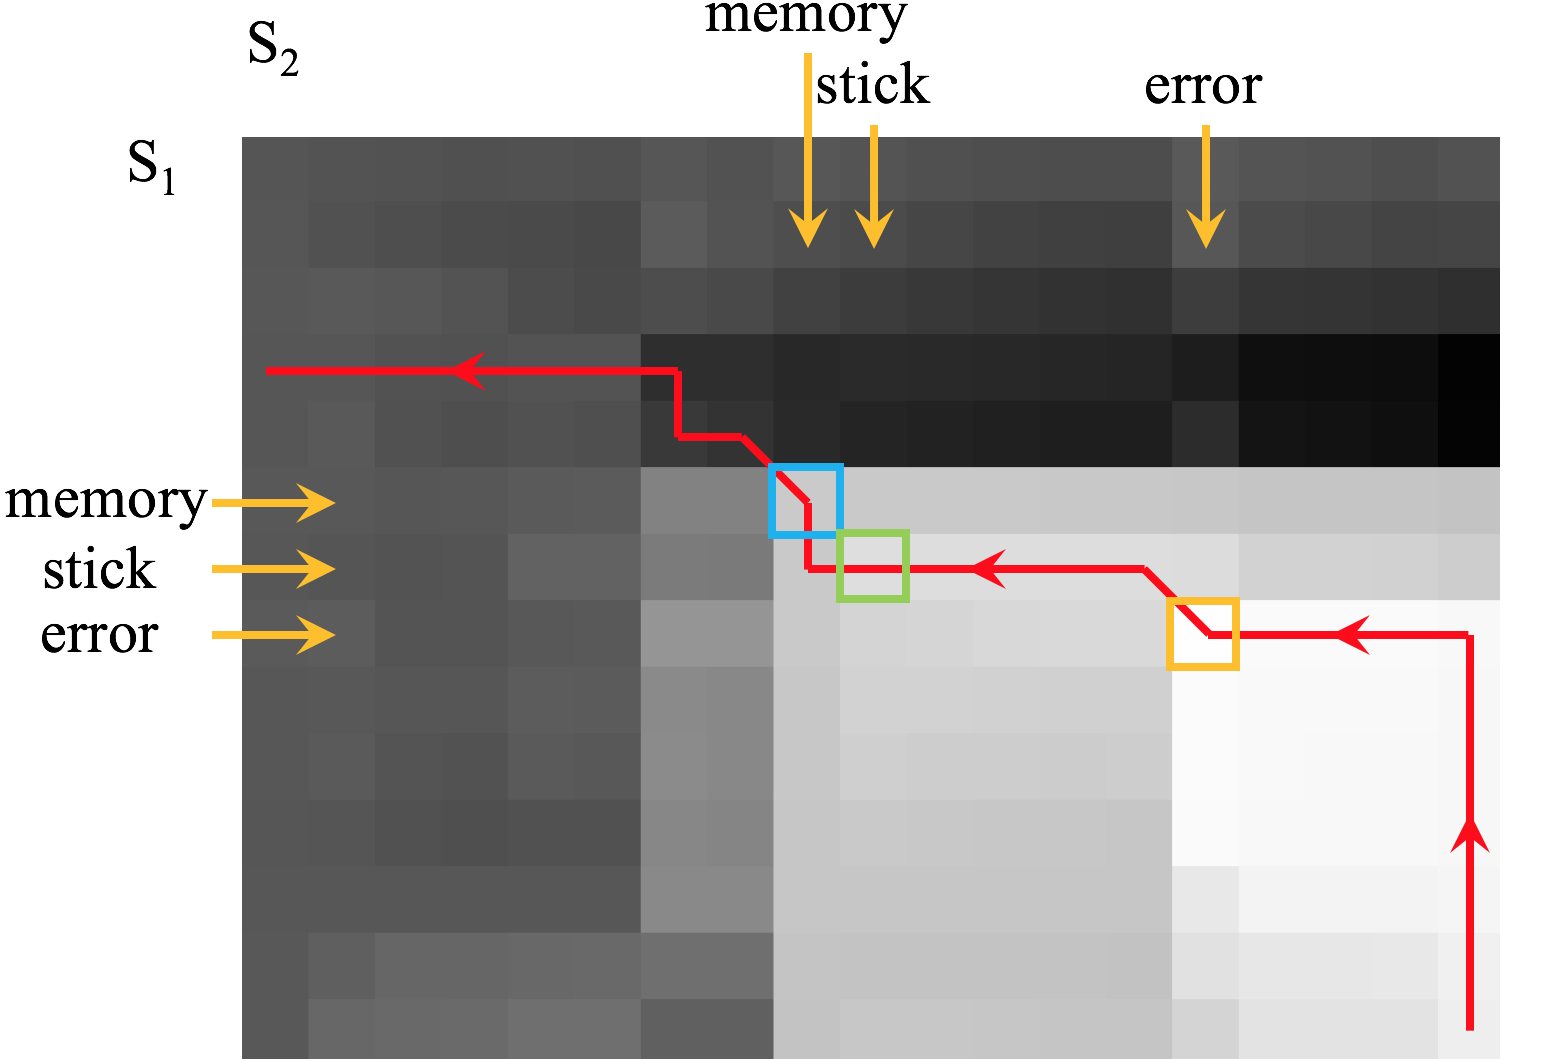
\includegraphics[width=0.7\textwidth]{figures/qa_path.png}
\caption{由Match-SRNN学习的代表性交互,亮度取决于每个位置的交互值,红色路径表示通过回溯最大门限生成的信息扩散过程。}
\label{fig:tensor}
\end{figure}

\textbf{结论}

在本文中,我们提出了一个递归思想来解决复杂的语义匹配问题。
具体而言,提出了一种新的深度学习体系结构,即Match-SRNN来对递归匹配结构进行建模。 匹配SRNN由三部分组成:获得单词级别交互的神经张量网络,递归地生成全局交互的空间RNN以及输出匹配度的线性评分函数。 我们的分析揭示了Match-SRNN与LCS的有趣联系。 最后,我们在语义匹配任务上的实验表明Match-SRNN可以显着优于现有的深度学习方法。 此外,我们通过一个真实的例子可视化了Match-SRNN发现的递归匹配结构。




